\part{Partial differential equations}
\section{Introduction}
\subsection*{General}
\begin{frame}[label=contents_pde]
  \frametitle{Today's outline}
  \mode<beamer>{
    \only<1>{\tableofcontents}
  }
  \only<2>{\tableofcontents[currentsection]}
\end{frame}

\begin{frame}
  \frametitle{Overview}
  \begin{block}{Main question}
  How to solve parabolic PDEs like:
  \[
    \frac{\partial c}{\partial t} = \mathcal{D}\frac{\partial^2 c}{\partial x^2} - u\frac{\partial c}{\partial x} + R
  \]
  with \quad
  \begin{minipage}{0.4\textwidth}
      \begin{align*}
        &t = 0; 0\leq x \leq \ell &\Rightarrow& c=c_0 \\
        &t > 0; x=0  &\Rightarrow& -\mathcal{D} \frac{\partial c}{\partial x} + uc = u_\text{in} c_\text{in}  \\
        &t > 0; x=\ell  &\Rightarrow& \frac{\partial c}{\partial x}=0 
      \end{align*}
  \end{minipage} \\ \vskip1em
  accurately and efficiently?
  \end{block}
\end{frame}

\begin{frame}
  \frametitle{What is a PDE?}
    \begin{block}{Partial differential equation}
      An equation containing a function and their derivatives to multiple independent variables.
    \end{block}
    \begin{block}{Order of PDE}
      The highest derivative appearing in the PDE
    \end{block}
    \pause
    General second order PDE:
    \[
      A \frac{\partial^2 f}{\partial x^2} + B\frac{\partial^2 f}{\partial x \partial y} + C\frac{\partial^2 f}{\partial y^2} + D\frac{\partial f}{\partial x} + E\frac{\partial f}{\partial y} +Ff = G
    \]
    \begin{itemize}
      \item Linear equation: Coefficients $A,B,\ldots,G$ do not depend on $x$ and $y$.
      \item Non-linear equation: Coefficients $A,B,\ldots,G$ are a function of $x$ and $y$.
    \end{itemize}
\end{frame}

\begin{frame}
  \frametitle{Classification of PDE's}
  \footnotesize\selectfont
  $\displaystyle A \frac{\partial^2 f}{\partial x^2} + B\frac{\partial^2 f}{\partial x \partial y} + C\frac{\partial^2 f}{\partial y^2} + D\frac{\partial f}{\partial x} + E\frac{\partial f}{\partial y} +Ff = G
  $ \\
  The discriminant $\Delta$ of a quadratic polynomial is computed as (note: only the higher order coefficients are important):\\
  $\displaystyle \Delta = B^2 -4AC$
  \pause
  \begin{itemize}
   \colorize<2> \item $\displaystyle \Delta < 0 \Rightarrow$ Elliptic equation \\
    (e.g. Laplace equation for stationary diffusion in 2D)
   \colorize<3> \item $\displaystyle \Delta = 0 \Rightarrow$ Parabolic equation \\
    (e.g. instationary heat penetration in 1D)
  \colorize<4> \item $\displaystyle \Delta > 0 \Rightarrow$ Hyperbolic equation \\
    (e.g. wave equation)
  \end{itemize}
  \begin{columns}
    \column{0.33\textwidth}
    \onslide<2->{
      \begin{center}
        \begin{tikzpicture}
          \begin{axis}[width=1.2\columnwidth,height=4cm,
            ymin=0,ymax=5,xmin=0,xmax=5,
            ticks=none,axis x line=bottom,axis y line=left
            axis background/.style={fill=white},
            axis x line=middle,axis y line=middle,ylabel=$y$,xlabel=$x$]
            \draw (axis cs:2.5,2.3) ellipse [x radius=120, y radius=150];
          \end{axis}
        \end{tikzpicture}
      \end{center}
    }
    \column{0.33\textwidth}
    \onslide<3->{
      \begin{center}
        \begin{tikzpicture}<3>
          \begin{axis}[width=1.2\columnwidth,height=4cm,
            ymin=0,ymax=5,xmin=0,xmax=5,
            ticks=none,axis x line=bottom,axis y line=left
            axis background/.style={fill=white},
            axis x line=middle,axis y line=middle,ylabel=$y$,xlabel=$x$]
            \addplot[smooth,domain=1:4] {1.2857*x^2 -6.4286*x+9.15};
          \end{axis}
        \end{tikzpicture}
      \end{center}
    }
    \column{0.33\textwidth}
    \onslide<4>{
      \begin{center}
        \begin{tikzpicture}
          \begin{axis}[width=1.2\columnwidth,height=4cm,
            ymin=0,ymax=5,xmin=0,xmax=5,
            ticks=none,axis x line=bottom,axis y line=left
            axis background/.style={fill=white},
            axis x line=middle,axis y line=middle,ylabel=$y$,xlabel=$x$]
            \addplot[smooth,domain=1:4] {4/x};
          \end{axis}
        \end{tikzpicture}
      \end{center}
    }
  \end{columns}
  \vfill
\end{frame}

\begin{frame}
  \frametitle{Importance of classification}
  Different PDE types require different solution techniques because of the difference in range of influence:
  \begin{itemize}
    \colorize<2> \item \emph{Characteristics} \\
    Curves in $xy$-domain along with signal propagation takes place
    \colorize<3> \item \emph{Domain of dependence of point $P$} \\
    points in $xy$-domain which influence the value of $f$ in point $P$
    \colorize<4> \item \emph{Range of influence of point $P$}\\
    points in $xy$-domain which are influenced by the value of $f$ in point $P$
  \end{itemize}
\end{frame}

\begin{frame}
  \frametitle{Example elliptic PDE (boundary value problems: BVP)}
  \begin{columns}
    \column{0.65\textwidth}
    \begin{center}
      \begin{tikzpicture}[scale=0.7]
      \foreach \x in {0,...,6}
        \foreach \y in {0,...,4} 
          {
    %        \pgfmathtruncatemacro{\label}{\x - 5 *  \y +21}
          \ifthenelse{\x=0 \OR \x=6 \OR \y=0 \OR \y=4}{\node [gdot,fill=tuered]  (\x\y) at (1.5*\x,1.5*\y) {};}
          \node [gdot,fill=tueblue]  (\x\y) at (1.5*\x,1.5*\y) {};} 

        \foreach \x [count=\xi] in {0,...,5}
          \foreach \y [count=\yi] in {0,...,3}  
            \draw (\x\y)--(\x\yi)-- (\xi\yi)--(\xi\y)--(\x\y);% (\y\x)--(\yi\x) ;
      \end{tikzpicture}
    \end{center}
    \column{0.35\textwidth}
    \tikz{\node [gdot,fill=tueblue] {};} Grid point at which dependent variable has to be computed \\
    \tikz{\node [gdot,fill=tuered] {};}  Grid point at which boundary condition is specified
  \end{columns} \vskip1em
  Typical example: Poisson equation
  \[
    \frac{\partial^2 T}{\partial x^2}+\frac{\partial^2 T}{\partial y^2}= f(x,y)
  \]
  Efficiency (memory requirements, CPU time) of the numerical method is of crucial importance.
\end{frame}

\begin{frame}
  \frametitle{Example parabolic PDE (initial value problem: IVP)}
  \begin{columns}
    \column{0.65\textwidth}
    \begin{center}
      \begin{tikzpicture}[scale=0.7]
      \foreach \x in {0,...,6}
        \foreach \y in {0,...,4} 
          {
    %        \pgfmathtruncatemacro{\label}{\x - 5 *  \y +21}
          \ifthenelse{\x=0 \OR \x=6 \OR \y=0}{\node [gdot,fill=tuered]  (\x\y) at (1.5*\x,1.5*\y) {};}
          \node [gdot,fill=tueblue]  (\x\y) at (1.5*\x,1.5*\y) {};} 

        \foreach \x [count=\xi] in {0,...,5}
          \foreach \y [count=\yi] in {0,...,3}  
            \draw (\x\y)--(\x\yi)-- (\xi\yi)--(\xi\y)--(\x\y);% (\y\x)--(\yi\x) ;
      \end{tikzpicture}
    \end{center}
    \column{0.35\textwidth}
    \tikz{\node [gdot,fill=tueblue] {};} Grid point at which dependent variable has to be computed \\
    \tikz{\node [gdot,fill=tuered] {};}  Grid point at which boundary condition is specified
  \end{columns} \vskip1em
  Typical example: Poisson equation
  \[
    \frac{\partial c}{\partial t} + u\frac{\partial c}{\partial x} = \mathcal{D}\frac{\partial^2 c}{\partial x^2}  + R
  \]
  Stability (in numerical sense) of the numerical method is of crucial importance.
\end{frame}

\begin{frame}
  \frametitle{Boundary conditions}
  \begin{itemize}
   \colorize<1> \item Dirichlet or fixed condition: prescribed value of $f$ at boundary
    \[
      f = f_0 \qquad\text{$f_0$ is a known function}
    \]
   \colorize<2> \item Neumann condition: prescribed value of derivative of $f$ at boundary
    \[
      \frac{\partial f}{\partial n} = q \qquad\text{$q$ is a known function}
    \]
    \colorize<3> \item Mixed or Robin condition: relation between $f$ and $\frac{\partial f}{\partial n}$ at boundary
    \[
      a\frac{\partial f}{\partial n} + bf = c \qquad\text{$a$, $b$ and $c$ are known functions}
    \]
  \end{itemize}
\end{frame}

\begin{frame}
  \frametitle{Numerical solution method}
  Finite differences (method of lines, MOL):
  \begin{enumerate}
    \item Discretize spatial domain in discrete grid points
    \item Find suitable approximation for the spatial derivatives
    \item Substitute approximations in PDE, which gives a system of ODE's, one for every grid points
    \item Advance in time with a suitable ODE solver
  \end{enumerate}
  \vskip2em
  Alternative methods: collocation, Galerkin or Finite Element methods
\end{frame}

\section{Instationary diffusion equation}
\subsection{Discretization}
\againframe<2>{contents_pde}
\begin{frame}
  \frametitle{Instationary diffusion equation (Fick's second law)}
  \footnotesize\selectfont
  $ \displaystyle
    \frac{\partial c}{\partial t} = \mathcal{D} \frac{\partial^2 c}{\partial x^2},\quad \text{with}\quad$  \begin{minipage}{0.6\textwidth}
     $t = 0; 0\leq x \leq \ell \Rightarrow c=c_0$\\
     $t > 0; x=0  \Rightarrow c=c_L$\\
     $t > 0; x=\ell  \Rightarrow c=c_R$
  \end{minipage} \\ \vskip1em
  Second derivative $\displaystyle \frac{\partial^2c}{\partial x^2}$ \quad
  \begin{tikzpicture}[scale=2]
  \node[fdot] (c0) at (0,0) {};
  \node[fdot] (c1) at (1,0) {};
  \node[fdot] (c2) at (2,0) {};
  \draw[line] (c0) -- (c1) -- (c2);
  \node[above] (t0) at (c0) {$c_{i-1}$};
  \node[above] (t1) at (c1) {$c_{i}$};
  \node[above] (t2) at (c2) {$c_{i+1}$};
  \end{tikzpicture}
  \onslide<2->{
    \begin{align*}
      c_{i+1} &= c_i + \left. \frac{\partial c}{\partial x}\right|_i \Delta x + \frac{1}{2} \left. \frac{\partial^2 c}{\partial x^2} \right|_i \Delta x^2 + \frac{1}{6} \left. \frac{\partial^3 c}{\partial x^3}\right|_i \Delta x^3 + \ldots & \\
      c_{i-1} &= c_i - \left. \frac{\partial c}{\partial x}\right|_i \Delta x + \frac{1}{2} \left. \frac{\partial^2 c}{\partial x^2} \right|_i \Delta x^2 - \frac{1}{6} \left. \frac{\partial^3 c}{\partial x^3}\right|_i \Delta x^3 + \ldots & \phantom{+}\\
        \cline{1-3} \onslide<3->{
        c_{i+1} + c_{i-1} &= 2c_i + \left. \frac{\partial^2 c}{\partial x^2} \right|_i \Delta x^2 + \mathcal{O}{(\Delta x^4)} & \\
        \Rightarrow \left. \frac{\partial^2 c}{\partial x^2} \right|_i &= \frac{c_{i+1} - 2c_i + c_{i-1}}{\Delta x^2} + \mathcal{O}{(\Delta x^2)} &
      }
    \end{align*}
  \onslide<4>{\centering\tikz{\node[emphblock]{Due to symmetric discretization: second order (central discretization).};}}
  }
  
\end{frame}

\begin{frame}
  \frametitle{Instationary diffusion equation (Fick's second law)}
  \small\selectfont
  An alternative discretization: \\
  $\displaystyle \left. \frac{\partial^2 c}{\partial x^2} \right|_i = \frac{\left. \frac{\partial c}{\partial x}\right|_{i+\frac{1}{2}} - \left. \frac{\partial c}{\partial x}\right|_{i-\frac{1}{2}}}{\Delta x} + \mathcal{O}{(\Delta x^2)} $ \quad
    \begin{tikzpicture}[scale=2]
  \node[fdot] (c0) at (0,0) {};
  \node[fdot] (c1) at (1,0) {};
  \node[fdot] (c2) at (2,0) {};
  \draw[line] (c0) -- node[midway,cross] (d1) {} (c1) -- node[midway,cross] (d2) {} (c2);
  \node[above] (t0) at (c0) {$c_{i-1}$};
  \node[above] (t1) at (c1) {$c_{i}$};
  \node[above] (t2) at (c2) {$c_{i+1}$};
  \node[above] (t3) at (d1) {$\left. \frac{\partial c}{\partial x}\right|_{i-\frac{1}{2}}$};
  \node[above] (t3) at (d2) {$\left. \frac{\partial c}{\partial x}\right|_{i+\frac{1}{2}}$};
  \end{tikzpicture} 
  \pause
  \[
    = \frac{\dfrac{c_{i+1}-c_{i}}{\Delta x} - \dfrac{c_{i}-c_{i-1}}{\Delta x}}{\Delta x} =  \frac{c_{i+1} - 2c_i + c_{i-1}}{\Delta x^2}
  \]
  \pause
  This is convenient for the derivation of $\displaystyle \frac{\partial}{\partial x}\left(\mathcal{D}\frac{\partial c}{\partial x}\right)$:
%   \hspace*{-2em}
  \begin{flalign*}
    \frac{\partial}{\partial x}\left(\mathcal{D}\frac{\partial c}{\partial x}\right) 
    &= \frac{\left. \mathcal{D}_{i+\frac{1}{2}} \frac{\partial c}{\partial x}\right|_{i+\frac{1}{2}} - \left. \mathcal{D}_{i-\frac{1}{2}}\frac{\partial c}{\partial x}\right|_{i-\frac{1}{2}}}{\Delta x}
    = \frac{\mathcal{D}_{i+\frac{1}{2}} \dfrac{c_{i+1}-c_{i}}{\Delta x} - \mathcal{D}_{i-\frac{1}{2}}\dfrac{c_{i}-c_{i-1}}{\Delta x}}{\Delta x} & \\
    &= \frac{\mathcal{D}_{i+\frac{1}{2}}c_{i+1} - \left( \mathcal{D}_{i+\frac{1}{2}} + \mathcal{D}_{i-\frac{1}{2}}\right) c_i + \mathcal{D}_{i-\frac{1}{2}} c_{i-1}}{(\Delta x)^2} &
  \end{flalign*}

\end{frame}

\begin{frame}
  \frametitle{Instationary diffusion equation (Fick's second law)}
  $\displaystyle \frac{\partial^2f}{\partial x^2}$ \qquad
    \begin{tikzpicture}[scale=3]
  \node[fdot] (c0) at (0,0) {};
  \node[fdot] (c1) at (1,0) {};
  \node[fdot] (c2) at (2,0) {};
  \draw[line] (c0) -- node[midway,cross] (d1) {} (c1) -- node[midway,cross] (d2) {} (c2);
  \node[above] (t0) at (c0) {$i-1$};
  \node[above] (t1) at (c1) {$i$};
  \node[above] (t2) at (c2) {$i+1$};
  \node[above] (t3) at (d1) {$i-\frac{1}{2}$};
  \node[above] (t3) at (d2) {$i+\frac{1}{2}$};
  \end{tikzpicture}
  \pause
  \begin{align*}
  f_{i+\frac{1}{2}} &= f_i + \frac{1}{2}\Delta x \left. \frac{\partial f}{\partial x}\right|_i \Delta x + \frac{1}{2}\left(\frac{1}{2}\Delta x\right)^2 \left. \frac{\partial^2 f}{\partial x^2} \right|_i +   \mathcal{O}{(\Delta x^3)}& \\
  f_{i-\frac{1}{2}} &= f_i - \frac{1}{2}\Delta x \left. \frac{\partial f}{\partial x}\right|_i \Delta x + \frac{1}{2}\left(\frac{1}{2}\Delta x\right)^2 \left. \frac{\partial^2 f}{\partial x^2} \right|_i +   \mathcal{O}{(\Delta x^3)}& \phantom{+}\\
    \cline{1-3}
    f_{i+\frac{1}{2}} -f_{i-\frac{1}{2}} &= \Delta x \frac{\partial f}{\partial x} + \mathcal{O}{(\Delta x^3)} & 
  \end{align*}
  \pause
  \[
    \Rightarrow \left. \frac{\partial f}{\partial x}\right|_i = \frac{f_{i+\frac{1}{2}} - f_{i-\frac{1}{2}}}{\Delta x} +  \mathcal{O}{(\Delta x^2)}
  \]
  Symmetric discretization yields second order!
\end{frame}

\begin{frame}
  \frametitle{Instationary diffusion equation: spatial discretization}
  Substitution of spatial derivatives yields:
  \[
    \frac{d c_i}{dt} = \mathcal{D} \frac{c_{i-1}-2c_i+c_{i+1}}{\Delta x^2} \quad \text{for}\, i=0,\ldots,N
  \]
  For example, using 6 (ridiculously low number!) grid points:\\ \pause \vskip1em
  \begin{tikzpicture}[scale=1.8]
  \foreach \x in {0,...,5}
    \node[fdot,label=$c_\x$] (c\x) at (\x,0) {};
  \draw[line,-] (c0)--(c1)--(c2)--(c3)--(c4)--(c5);
  \node<3->[emphblock,below=2em] (f0) at (c0) {$\phantom{\frac{c_0}{x^2}}c_0 = c_L \phantom{\frac{c_0}{x^2}}$};
  \draw<3-> (c0) -- (f0.north);
  \node<4->[emphblock,below=5em] (f1) at (c1) {$\frac{dc_1}{dt} = \mathcal{D}\frac{c_0-2c_1+c_2}{\Delta x^2}$};
  \draw<4-> (c1) -- (f1.north);
  \node<5->[emphblock,below=8em] (f2) at (c2) {$\frac{dc_2}{dt} = \mathcal{D}\frac{c_1-2c_2+c_3}{\Delta x^2}$};
  \draw<5-> (c2) -- (f2.north);
  \node<5->[emphblock,below=5em] (f3) at (c3) {$\frac{dc_3}{dt} = \mathcal{D}\frac{c_2-2c_3+c_4}{\Delta x^2}$};
  \draw<5-> (c3) -- (f3.north);
  \node<5->[emphblock,below=8em] (f4) at (c4) {$\frac{dc_4}{dt} = \mathcal{D}\frac{c_3-2c_4+c_5}{\Delta x^2}$};
  \draw<5-> (c4) -- (f4.north);
  \node<5->[emphblock,below=2em] (f5) at (c5) {$\phantom{\frac{c_0}{x^2}} c_5 = c_R \phantom{\frac{c_0}{x^2}}$};
  \draw<5-> (c5) -- (f5.north);
  \node (p) at (-0.6,-12) {};
  \end{tikzpicture}
\end{frame}

\begin{frame}
  \frametitle{Instationary diffusion equation: boundary conditions}
  Two options:
  \begin{enumerate}
    \colorize<1> \item Keep boundary conditions as additional equations:
    \begin{multline*}
      c_0 = c_L, \frac{dc_1}{dt} = \mathcal{D}\frac{c_0-2c_1+c_2}{\Delta x^2},\frac{dc_2}{dt} = \mathcal{D}\frac{c_1-2c_2+c_3}{\Delta x^2},\\ 
      \frac{dc_3}{dt} = \mathcal{D}\frac{c_2-2c_3+c_4}{\Delta x^2},\frac{dc_4}{dt} = \mathcal{D}\frac{c_3-2c_4+c_5}{\Delta x^2},c_5 = c_R
    \end{multline*}
    \colorize<2> \item Substitute boundary conditions to reduce number of equations:
    \begin{multline*}
      \frac{dc_1}{dt} = \mathcal{D}\frac{{\color<2>{tuered}c_L}-2c_1+c_2}{\Delta x^2},\frac{dc_2}{dt} = \mathcal{D}\frac{c_1-2c_2+c_3}{\Delta x^2},\\ 
      \frac{dc_3}{dt} = \mathcal{D}\frac{c_2-2c_3+c_4}{\Delta x^2},\frac{dc_4}{dt} = \mathcal{D}\frac{c_3-2c_4+{\color<2>{tuered}c_R}}{\Delta x^2}
    \end{multline*}
  \end{enumerate}
\end{frame}

\begin{frame}[t]
  \frametitle{Instationary diffusion equation: temporal discretization}
  $\displaystyle  \frac{d c_i}{dt} = \mathcal{D} \frac{c_{i-1}-2c_i+c_{i+1}}{\Delta x^2} $\\
  \begin{block}{Time discretization: forward Euler (explicit)}
    \begin{multline*}
      \frac{c_i^{{\color{tuered}n+1}}-c_i^{{\color{tuered}n}}}{\Delta t} = \mathcal{D} \frac{c_{i-1}^{{\color{tuered}n}}-2c_i^{{\color{tuered}n}}+c_{i+1}^{{\color{tuered}n}}}{\Delta x^2} \\
	\Rightarrow c_i^{n+1} = \Fo c_{i-1}^n + (1-2\Fo)c_i^n + \Fo c_{i+1}^n \quad \text{with}\, \Fo=\frac{\mathcal{D}\Delta t}{\Delta x^2}
    \end{multline*}
  \end{block}
  \vskip1em
  Straightforward updating (explicit equation), simple to implement in a program but stability constraint $\Fo = \frac{\mathcal{D}\Delta t}{\Delta x^2} < \frac{1}{2}$!\\ \vskip1ex
  Small $\Delta x \Rightarrow$ small $\Delta t \Rightarrow$ patience required \frownie{} 
\end{frame}

\begin{frame}[t]
  \frametitle{Instationary diffusion equation: temporal discretization}
  $\displaystyle \frac{d c_i}{dt} = \mathcal{D} \frac{c_{i-1}-2c_i+c_{i+1}}{\Delta x^2}$\\
  \begin{block}{Time discretization: backward Euler (implicit)}
    \begin{multline*}
      \frac{c_i^{{\color{tuered}n+1}}-c_i^{{\color{tuered}n}}}{\Delta t} = \mathcal{D} \frac{c_{i-1}^{{\color{tuered}n+1}}-2c_i^{{\color{tuered}n+1}}+c_{i+1}^{{\color{tuered}n+1}}}{\Delta x^2} \\
	\Rightarrow -\Fo c_{i-1}^{n+1} + (1+2\Fo)c_i^{n+1} - \Fo c_{i+1}^{n+1} = c_i^{n} \quad \text{with}\, \Fo=\frac{\mathcal{D}\Delta t}{\Delta x^2}
    \end{multline*}
  \end{block}
  \vskip1em
  Requires the solution of a system of linear equations, but no stability constraints!
  \vskip1em
  {\scriptsize Note: extension to higher order schemes (with time step adaptation) straightforward. Often second or third order optimal, because for each Euler-like step in the additional order an often large system needs to be solved (not treated in this course).}
\end{frame}

\subsection{Solving the diffusion equation}
\begin{frame}
  \frametitle{Solving the instationary diffusion equation: example}
  \tikz \node[emphblock,text width=\textwidth] {
    Solve the diffusion problem using explicit discretization: \\ \vskip1ex
    $ \displaystyle \frac{\partial c_i}{\partial t} = \mathcal{D}\frac{\partial^2 c}{\partial x^2}\quad $  with\quad 
    \begin{minipage}{0.6\textwidth}
      $0\leq x \leq \delta$, $\delta = 5\cdot10^{-3}$ \si{\meter} \\
      $\delta/\Delta x = 100$ grid cells \\
      $\mathcal{D}=1\cdot10^{-8}$ \si{\meter\squared\per\second} \\
      $t_\text{end} = 5000$ \si{\second}\\
      $c_\text{L} = 1$ \si{\mol\per\cubic\meter}
      $c_\text{R} = 0$ \si{\mol\per\cubic\meter}
    \end{minipage}
  };
  \pause\vskip1em
  $c_i^{n+1} = \Fo c_{i-1}^n + (1-2\Fo)c_i^n + \Fo c_{i+1}^n \quad \text{with}\, \Fo=\frac{\mathcal{D}\Delta t}{\Delta x^2}$
  \pause\vskip1em
  \begin{enumerate}
    \item Initialise variables
    \item Compute time step so that $\Fo \leq \frac{1}{2} \Rightarrow \Delta t = 0.125 \si{\second}$!
    \item Compute 40000 time steps times 100 grid nodes!
    \item Store solution
  \end{enumerate}
\end{frame}

\begin{frame}[fragile]
  \frametitle{Solving the instationary diffusion equation: example}
  Initialise the variables and matrices:
  \begin{lstlisting}[basicstyle=\scriptsize\ttfamily]
Nx = 100;           % Nc grid points
Nt = 40000;         % Nt time steps
D = 1e-8;           % m/s
c_L = 1.0; c_R = 0; % mol/m3
t_end = 5000.0;     % s
x_end = 5e-3;       % m

% Time step and grid size
dt = t_end/Nt; 
dx = x_end/Nx;

% Fourier number
Fo=D*dt/dx/dx

% Initial matrices for solutions (Nx times Nt)
c = zeros(Nt+1,Nx+1);  % All concentrations are zero
c(:,1)  = c_L;     % Concentration at left side
c(:,Nx+1) = c_R;     % Concentration at right side

% Grid node and time step positions
x = linspace(0,x_end,Nx+1);
  \end{lstlisting}
\end{frame}

\begin{frame}<handout:0>[fragile]
  \frametitle{Solving the instationary diffusion equation: example}
  Compute the solution (nested time-and-grid loop):
  \begin{lstlisting}
for n = 1:Nt % time loop
    for i = 2:Nx % Nested loop for grid nodes
        c(n+1,i) = Fo*c(n,i-1) + (1-2*Fo)*c(n,i) + Fo*c(n,i+1);
    end
end
  \end{lstlisting}
  \pause
  Plotting the solution at $t=\left\{12.5,62.5,125,625,5000\right\}$ \si{\second}:\\
  \begin{columns}[T]
  \column{0.4\textwidth}
    \begin{lstlisting}
% Output times
outt = [12.5 62.5 125 625 5000];

% Convert+round to time steps
outt_dt = fix(outt/dt);

% Plot all time steps at once
plot(x,c(outt_dt,:))
  \end{lstlisting}
  \column{0.6\textwidth}
      \begin{tikzpicture}
        \begin{axis}[every axis/.append style={font=\tiny},
          width=\columnwidth, height=5cm,     % size of the image
          grid = major,
          grid style={dashed, gray!30},
          ymax=1,ymin=0,xmax=5e-3,xmin=0,
          axis background/.style={fill=white},
          ylabel={$c$ [\si{\mol\per\cubic\meter}]},xlabel={$x$ [\si{\meter}]},ylabel near ticks]

          % Actual equation
          \addplot[graph,draw=tuered] table [y index={1}] {data/diff_explicit.dat};
          \addplot[graph,draw=tuelblue] table [y index={2}] {data/diff_explicit.dat};
          \addplot[graph,draw=tuegreen] table [y index={3}] {data/diff_explicit.dat};
          \addplot[graph,draw=tueorange] table [y index={4}] {data/diff_explicit.dat};
          \addplot[graph,draw=tuedblue] table [y index={5}] {data/diff_explicit.dat};
        \end{axis}    
      \end{tikzpicture}
  \end{columns}
\end{frame}

\begin{frame}<handout:1|beamer:0>[fragile]
  \frametitle{Solving the instationary diffusion equation: example}
  Compute the solution (nested time-and-grid loop):
  \begin{itemize}
      \item Create a time-loop
      \item Create a loop over \emph{internal} grid points
      \item Update each node using $c_i^{n+1} = \Fo c_{i-1}^n + (1-2\Fo)c_i^n + \Fo c_{i+1}^n$
      \item Plot the solution for selected time steps
  \end{itemize}
  \pause
  Plotting the solution at $t=\left\{12.5,62.5,125,625,5000\right\}$ \si{\second}.
      \begin{tikzpicture}
        \begin{axis}[every axis/.append style={font=\tiny},
          width=\textwidth, height=4.5cm,     % size of the image
          grid = major,
          grid style={dashed, gray!30},
          ymax=1,ymin=0,xmax=5e-3,xmin=0,
          axis background/.style={fill=white},
          ylabel={$c$ [\si{\mol\per\cubic\meter}]},xlabel={$x$ [\si{\meter}]},ylabel near ticks]

          % Actual equation
          \addplot[graph,draw=tuered] table [y index={1}] {data/diff_explicit.dat};
          \addplot[graph,draw=tuelblue] table [y index={2}] {data/diff_explicit.dat};
          \addplot[graph,draw=tuegreen] table [y index={3}] {data/diff_explicit.dat};
          \addplot[graph,draw=tueorange] table [y index={4}] {data/diff_explicit.dat};
          \addplot[graph,draw=tuedblue] table [y index={5}] {data/diff_explicit.dat};
        \end{axis}    
      \end{tikzpicture}
\end{frame}

\begin{frame}[fragile]
  \frametitle{Solving the instationary diffusion equation: example}
  A double-loop can impose serious computation times if the number of grid points increases:
  \begin{lstlisting}
for n = 1:Nt-1 % time loop
    for i = 2:Nx % Nested loop for grid nodes
        c(n+1,i) = Fo*c(n,i-1) + (1-2*Fo)*c(n,i) + Fo*c(n,i+1);
    end
end
  \end{lstlisting}
Remedy: vectorization. Construct a 3-point stencil Laplacian matrix first, then use the matrix product to evolve the simulation:
\begin{lstlisting}
% Construct sparse matrix
e = ones(Nx-1,1);
md = [1; (1-2*Fo)*e; 1];
ld = [Fo*e; 0; 0];
ud = [0; 0; Fo*e;];
A = spdiags([ld md ud],[-1 0 1],Nx+1,Nx+1);

% Faster for row-wise operations, so transpose
c=c';
for n = 1:Nt-1 % time loop
    c(:,n+1) = A*c(:,n);
end
\end{lstlisting}
\end{frame}

\begin{frame}
  \frametitle{Solving the diffusion equation implicitly}
  \rowcolors{1}{}{}
%   \small\selectfont
  \tikz \node[emphblock]{Linear system $A\vec{x}=\vec{b}$ from $-\Fo c_{i-1}^{n+1} + (1+2\Fo)c_i^{n+1} - \Fo c_{i+1}^{n+1} = c_i^{n}$};
  \footnotesize\selectfont
  \[
    \begin{pmatrix}
      \color<2>{tuered}1       &  0      &  0      & 0       &\cdots &  0      \\
      \color<3>{tueblue}-\Fo    & \color<3>{tuered}(1+2\Fo)& \color<3>{tueblue}-\Fo    &0   & \cdots  &  0  \\
      0      &  \color<4>{tueblue}-\Fo   & \color<4>{tuered}(1+2\Fo)&\color<4>{tueblue}-\Fo     &\cdots &  0 \\
      0      &  0      & \color<5>{tueblue}-\Fo    & \color<5>{tuered}(1+2\Fo)& \cdots &  0 \\
      \vdots  & \vdots  & \vdots  & \vdots  &\ddots & \vdots  \\
      0       & 0       & 0       & 0       &\cdots & \color<6>{tuered}1
    \end{pmatrix} \cdot
    \begin{pmatrix}
      \color<3>{tueblue}\color<2>{tuered}c_0^{n+1} \\
      \color<4>{tueblue}\color<3>{tuered}c_1^{n+1} \\
      \color<3>{tueblue}\color<5>{tueblue}\color<4>{tuered}c_2^{n+1} \\
      \color<4>{tueblue}\color<5>{tuered}c_3^{n+1} \\
      \vdots \\
      \color<6>{tuered}c_m^{n+1} \\
    \end{pmatrix} = 
    \begin{pmatrix}
      \color<2>{tuered}c_0^{n} \\
      \color<3>{tuered}c_1^{n} \\
      \color<4>{tuered}c_2^{n} \\
      \color<5>{tuered}c_3^{n} \\
      \vdots \\
      \color<6>{tuered}c_m^{n} \\
    \end{pmatrix}
  \]
  \onslide<2->{$\displaystyle 1 \times c_0^{n+1} = c_0^n$ (boundary condition) \\ \vskip1ex}
  \onslide<3->{$\displaystyle -\Fo c_0^{n+1} + (1+2\Fo)c_1^{n+1} - \Fo c_2^{n+1} = c_1^n$ \\ \vskip1ex}
  \onslide<4->{$\displaystyle -\Fo c_1^{n+1} + (1+2\Fo)c_2^{n+1} - \Fo c_3^{n+1}  = c_2^n$ \\ \vskip1ex}
  \onslide<5->{$\displaystyle -\Fo c_2^{n+1} + (1+2\Fo)c_3^{n+1} - \Fo c_4^{n+1}  = c_3^n$ \\ \vskip1ex}
  \onslide<6->{$\displaystyle 1 \times c_m^{n+1} = c_m^n$ (boundary condition) \\ \vskip1ex}
\end{frame}

\begin{frame}<handout:1>[fragile]
  \frametitle{Solving the diffusion equation implicitly in Matlab}
  \rowcolors{1}{}{}
  To solve the linear system, we need to define matrix $A$. It is clear that storing many zeros is not efficient in terms of memory. We use a \emph{sparse matrix} format. Two alternative ways to set up the matrix:\\
  
  \begin{columns}[t]
  \column{0.45\textwidth}
  Set individual elements of the matrix:
  \begin{lstlisting}
% Bands in matrix (internal cells)
A = sparse(Nx+1,Nx+1);
for i=2:Nx
    A(i,i-1) = -Fo;
    A(i,i  ) = (1+2*Fo);
    A(i,i+1) = -Fo;
end

% Set boundary cells, only main diag:
A(1,1 ) = 1;        % Left
A(Nx+1,Nx+1) = 1;   % Right
  \end{lstlisting}
  \column{0.55\textwidth}
  Set matrix using bands:
    \begin{lstlisting}
% Bands in matrix (internal cells)
e = ones(Nx-1,1); % Ones for internal cells
md = [1; e*(1+2*Fo); 1]; % Main diagonal
ld = [-e*Fo; 0; 0]; % Lower diagonal
hd = [0; 0; -e*Fo;]; % Upper diagonal
A = spdiags([ld md hd],[-1 0 1],Nx+1,Nx+1)
  \end{lstlisting}
  Note: The first argument of \lstinline$spdiags$ defines each column as a diagonal, starting at row 1 (for lower-diagonal) or column 1 (for upper-diagonal).
  \end{columns}
\end{frame}

\begin{frame}[fragile]
  \frametitle{Solving the diffusion equation implicitly in Matlab}
  The command \lstinline$spy(A)$ shows a figure with the non-zero positions.
  \begin{center}
    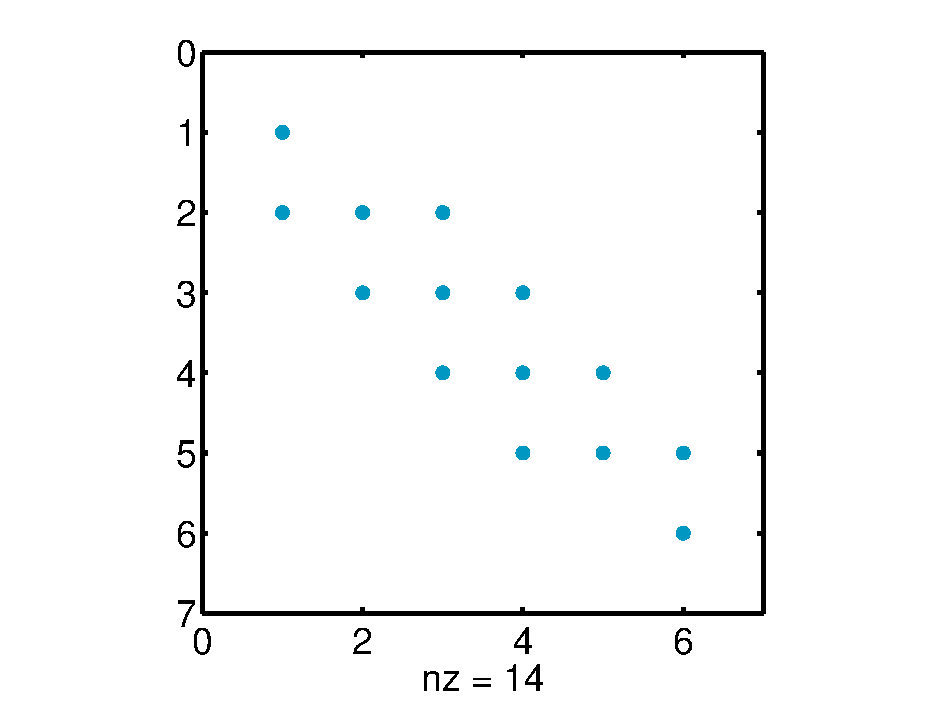
\includegraphics[width=0.65\textwidth]{spy-utc}
  \end{center}
\end{frame}

\begin{frame}<handout:1>[fragile]
  \frametitle{Solving the diffusion equation implicitly in Matlab}
  \rowcolors{1}{}{}
  The concentration matrix is initialised and the boundary conditions are set as follows:
  \begin{lstlisting}
% Initial matrices for solutions (Nx times Nt)
c = zeros(Nt+1,Nx+1);  % All concentrations are zero
c(:,1)    = c_L;       % Concentration at left side
c(:,Nx+1) = c_R;       % Concentration at right side
\end{lstlisting}
\vskip1em
The right hand side vector ($\vec{b}$) can now be set during the time-loop:
\begin{lstlisting}
for n = 1:Nt-1         % time loop 
    b = c(n,:)';       % Set right hand side
    solX = A\b;        % Solve linear system
    c(n+1,:) = solX;   % Store solution each time step
end
  \end{lstlisting}
\end{frame}

\begin{frame}[fragile]
  \frametitle{Solving the diffusion equation implicitly in Matlab}
  Plotting the solution at $t=\left\{12.5,62.5,125,625,5000\right\}$ \si{\second}.
      \begin{tikzpicture}
        \begin{axis}[every axis/.append style={font=\tiny},
          width=\textwidth, height=7.5cm,     % size of the image
          grid = major,
          grid style={dashed, gray!30},
          ymax=1,ymin=0,xmax=5e-3,xmin=0,
          axis background/.style={fill=white},
          ylabel={$c$ [\si{\mol\per\cubic\meter}]},xlabel={$x$ [\si{\meter}]},ylabel near ticks]

          % Actual equation
          \addplot[graph,draw=tuered] table [y index={1}] {data/diff_implicit.dat};
          \addplot[graph,draw=tuelblue] table [y index={2}] {data/diff_implicit.dat};
          \addplot[graph,draw=tuegreen] table [y index={3}] {data/diff_implicit.dat};
          \addplot[graph,draw=tueorange] table [y index={4}] {data/diff_implicit.dat};
          \addplot[graph,draw=tuedblue] table [y index={5}] {data/diff_implicit.dat};
        \end{axis}    
      \end{tikzpicture}
\end{frame}

\begin{frame}
  \frametitle{About explicit vs. implicit solutions}
  \begin{itemize}
    \item Explicit solution:
    \begin{itemize}
      \item Easy to implement
      \item Very small time steps required.
      \item This problem took about 0.5 \si{\second}.
    \end{itemize}
    \item Implicit solution:
    \begin{itemize}
      \item Harder to implement, needs sparse matrix solver
      \item No stability constraint
      \item This problem took about 0.05 \si{\second}
    \end{itemize}
    \item The difference will become much larger for systems with e.g. more grid nodes!
  \end{itemize}
\end{frame}

\subsection{Non-linear source terms}
\begin{frame}
  \frametitle{Extension with non-linear source terms}
  $ \frac{\partial c}{\partial t} = \mathcal{D}\frac{\partial^2 c}{\partial x^2} + R(c) \quad \text{with}\quad$  \begin{minipage}{0.5\textwidth}
     $t = 0; 0\leq x \leq \ell \Rightarrow c=c_0$\\
     $t > 0; x=0  \Rightarrow c=c_L$\\
     $t > 0; x=\ell  \Rightarrow c=c_R$
  \end{minipage}
  \pause%\\ \vskip1em
  \begin{itemize}
    \item Forward Euler (explicit): simply add to right-hand side
    \begin{multline*}
      \frac{c_i^{n+1}-c_i^{n}}{\Delta t} = \mathcal{D} \frac{c_{i-1}^{{\color{tuered}n}}-2c_i^{{\color{tuered}n}}+c_{i+1}^{{\color{tuered}n}}}{\Delta x^2} + R(c_i^{{\color{tuered}n}}) \\ 
      \Rightarrow c_i^{n+1} = \Fo c_{i-1}^{n} + (1-2\Fo)c_i^n+\Fo c_{i+1}^n + R_i^n\Delta t
    \end{multline*}
    \pause
      \item Backward Euler (implicit): linearization required
  \end{itemize}
  \footnotesize
  \begin{flalign*}
  R(c_i^{n+1}) &= R(c_i^n)+ \left. \frac{dR}{dc}\right|_i^n (c_i^{n+1}-c_i^{n}) &&\\
  \frac{c_i^{n+1}-c_i^{n}}{\Delta t} &= \mathcal{D} \frac{c_{i-1}^{{\color{tuered}n+1}}-2c_i^{{\color{tuered}n+1}}+c_{i+1}^{{\color{tuered}n+1}}}{\Delta x^2} + R(c_i^{{\color{tuered}n+1}}) && \\ 
    \Rightarrow -\Fo c_{i-1}^{n+1} + (1&+2\Fo - \left. \frac{dR}{dc}\right|_i^n \Delta t)c_i^{n+1}-\Fo c_{i+1}^{n+1} = c_i^n + \left(R_i^n
    - \left. \frac{dR}{dc}\right|_i^n c_i^n\right)\Delta t && 
  \end{flalign*}
\end{frame}

\section{Convection}
\subsection{Discretization}
\againframe<2>{contents_pde}
\begin{frame}
  \frametitle{Extension with convection terms}
  \[
    \frac{\partial c}{\partial t} = \mathcal{D}\frac{\partial^2 c}{\partial x^2} - u\frac{\partial c}{\partial x} + R
  \]
  \vskip1em
  Discretization of first derivative $\dfrac{dc}{dx}$,\\
  looks simple but is numerical headache! \\ \vskip1em
  
  Central discretization: 
  \[
    \dfrac{dc}{dx} = \dfrac{c_{i+1}-c_{i-1}}{2\Delta x}
  \]
  $\Rightarrow$ simple and easy, too bad it doesn't work: yields unstable solutions if convection dominated.
\end{frame}

\subsection{Central difference scheme}
\begin{frame}
  \frametitle{Central difference scheme of 1st derivative}
  \small\selectfont
  \begin{columns}
    \column{0.35\textwidth}
      \tikz{\node[emphblock,text width=\columnwidth,minimum height=4.5em] {Unsteady convection:\\ \vskip0.5em $\displaystyle \frac{\partial c}{\partial t} = -u\frac{\partial c}{\partial x} $};}
    \column{0.65\textwidth}
      \tikz{\node[emphblock,text width=\columnwidth,minimum height=4.5em] {Central difference for first derivative:\\ \vskip0.5em$\displaystyle \frac{dc}{dx} = \frac{c_{i+1}-c_{i-1}}{2\Delta x}$};}
  \end{columns}
  \pause \vskip1em
  Forward Euler discretization of temporal and spatial domain:
  \begin{align*}
  \frac{c_i^{n+1}-c_i^{n}}{\Delta t} = -u\frac{c_{i+1}-c_{i-1}}{2\Delta x}
    \Rightarrow c_i^{n+1} = c_i^{n} -u\frac{c_{i+1}^n-c_{i-1}^n}{2\Delta x}\Delta t
  \end{align*}
  \onslide<3->{
    \begin{tikzpicture}
  %       \tikzset{at/.style=}
      \begin{axis}[every axis/.append style={font=\tiny},
        width=\textwidth, height=4.5cm,     % size of the image
        grid = major,
        grid style={dashed, gray!30},
        ymax=1.5,   % end   the diagram at this y-coordinate
        axis background/.style={fill=white},
        ylabel={$c$ [\si{\mol\per\cubic\meter}]},xlabel={$x$ [\si{\meter}]},ylabel near ticks]

        % Actual equation
        \only<3->{\addplot[graph,draw=tuered] table [y index={2}] {data/conv_cendiff.dat};}
        \only<3->{\addplot[graph,sharp plot,draw=tuered,dashed] table [y index={2}] {data/conv_ex.dat};}
        \only<4->{\addplot[graph,draw=tueblue] table [y index={4}] {data/conv_cendiff.dat};}
        \only<4->{\addplot[graph,sharp plot,draw=tueblue,dashed] table [y index={4}] {data/conv_ex.dat};}
        \only<5->{\addplot[graph,draw=tuegreen] table [y index={6}] {data/conv_cendiff.dat};}
        \only<5->{\addplot[graph,sharp plot,draw=tuegreen,dashed] table [y index={6}] {data/conv_ex.dat};}
      \end{axis} 
      \end{tikzpicture}
    }
\end{frame}

{\nologo
\begin{frame}
  \frametitle{Extension with convection terms}
  \rowcolors[]{20}{white}{white}
  Solution: upwind discretization, like CSTR's in series:
  \begin{center}
    \begin{tikzpicture}
      %     \draw[help lines] (0,0) grid (6,6);
      \foreach \x [count=\xi from 0,count=\ci from 1] in {0,1.5,3} {
        \draw[line,-,top color=white!80,bottom color=maincolor!80,] 
        (\x,2.5-\xi*0.5)[rounded corners=14pt]--  node[pos=0.42](in\xi){} (\x,1-\xi*0.5)  -- node[midway,below](m\xi) {$c_\ci$} (\x+1,1-\xi*0.5) [rounded corners=8pt] -- node[near start](out\xi){}(\x+1,2.5-\xi*0.5) --  cycle;
        \draw (\x+0.5,3-\xi*0.5) -- (\x+0.5,1.5-\xi*0.5);
        \draw (\x+0.4,1.5-\xi*0.5) ellipse [x radius=0.1, y radius=0.05];
        \draw (\x+0.6,1.5-\xi*0.5) ellipse [x radius=0.1, y radius=0.05];
        }
        
        \draw[line,<-] (in0.center) -- node[near end,above] {$c_L$} ++(-0.5,0);
        \draw[line,->] (out0.center) -- (in1.center);
      \draw[line,->] (out1.center) -- (in2.center);
      \draw[line,->] (out2.center) -- node[near end,above] {$c_R$}++(0.5,0);
    \end{tikzpicture}
  \end{center}
  First order upwind: 
  $\displaystyle \left.-u\frac{dc}{dx}\right|_i  = \left\{ 
  \begin{array}{l l}
    -u \dfrac{c_i-c_{i-1}}{\Delta x} & \quad \text{if $u\geq 0$}\\
    \phantom{.}\\
    -u \dfrac{c_{i+1}-c_i}{\Delta x} & \quad \text{if $u < 0$}\\
  \end{array} \right.$
  \pause
  Stable if $\text{Co} = \frac{u\Delta t}{\Delta x} < 1$ (with $\text{Co}$ the Courant number). However, only $1^\text{st}$ order accurate (large smearing of concentration fronts). Higher order upwind requires TVD schemes (trick of the trade)...
\end{frame}

\subsection{Upwind scheme}
\begin{frame}
  \frametitle{First order upwind scheme of 1st derivative}
  \small\selectfont
  \rowcolors{1}{}{}
  \begin{columns}[T]
    \column{0.35\textwidth}
    \tikz{\node[emphblock,text width=\columnwidth,minimum height=8em] {Unsteady convection:\\ \vskip0.5em $\displaystyle \frac{\partial c}{\partial t} = -u\frac{\partial c}{\partial x} $};}
    \column{0.65\textwidth}
    \tikz{\node[emphblock,text width=\columnwidth,minimum height=8em] {Upwind scheme for first derivative:\\ \vskip0.5em $\displaystyle \left.-u\frac{dc}{dx}\right|_i  = \left\{ 
      \begin{array}{l l}
    -u\dfrac{c_i-c_{i-1}}{\Delta x} & \quad \text{if $u\geq 0$}\\
    \phantom{.}\\
    -u\dfrac{c_{i+1}-c_i}{\Delta x} & \quad \text{if $u < 0$}\\
  \end{array} \right.$};}
\end{columns}
\pause \vskip1em
Forward Euler discretization of temporal and spatial domain:
\begin{align*}
  \frac{c_i^{n+1}-c_i^{n}}{\Delta t} &= -u\frac{c_{i+1}-c_{i-1}}{2\Delta x} \\
    \Rightarrow c_i^{n+1} &= \left\{ 
      \begin{array}{l l}
        c_i^{n} -u \Delta t \dfrac{c_i-c_{i-1}}{\Delta x} & \quad \text{if $u\geq 0$}\\
        \phantom{.}\\
        c_i^{n}-u \Delta t \dfrac{c_{i+1}-c_i}{\Delta x} & \quad \text{if $u < 0$}\\
      \end{array} \right.
    \end{align*}
  \end{frame}
  
  \begin{frame}
    \frametitle{Upwind scheme: example}
    \footnotesize\selectfont
    Unsteady convection through a pipe:\\
    $ \displaystyle \frac{\partial c}{\partial t} = -u\frac{\partial c}{\partial x} \quad \text{with} \quad u=0.1 \si{\meter\per\second} \Rightarrow c_i^{n+1} = c_i^{n} -u\dfrac{c_i-c_{i-1}}{\Delta x}\Delta t$
    \begin{columns}
      \column{0.5\textwidth}
      \onslide<2->{
        \begin{center}
          Using 100 grid cells
	\vskip1ex
	\hspace*{-1cm}
	\begin{tikzpicture}
	  \begin{axis}[every axis/.append style={font=\tiny},
	    width=\columnwidth, height=4cm, grid = major,grid style={dashed, gray!30},axis background/.style={fill=white},
	    ymax=1.2,ylabel={$c$ [\si{\mol\per\cubic\meter}]},xlabel={$x$ [\si{\meter}]},ylabel near ticks,xlabel near ticks]
      
	    \only<2->{\addplot[graph,draw=tuered] table [y index={2}] {data/conv_upwind1.dat};}
	    \only<2->{\addplot[graph,sharp plot,draw=tuered,dashed] table [y index={2}] {data/conv_ex.dat};}
	    \only<3->{\addplot[graph,draw=tueblue] table [y index={4}] {data/conv_upwind1.dat};}
	    \only<3->{\addplot[graph,sharp plot,draw=tueblue,dashed] table [y index={4}] {data/conv_ex.dat};}
	    \only<4->{\addplot[graph,draw=tuegreen] table [y index={6}] {data/conv_upwind1.dat};}
	    \only<4->{\addplot[graph,sharp plot,draw=tuegreen,dashed] table [y index={6}] {data/conv_ex.dat};}
	  \end{axis} 
	\end{tikzpicture}
	\vskip1em
  \begin{tikzpicture}[scale=0.35,myshade/.style={left color=maincolor!80,right color=white!80,fill opacity=0.5},myfill/.style={fill=maincolor!80,fill opacity=0.5}]
    \shade[myshade] (0,0) arc (270:90:0.5 and 1.5) -- (8.5,3) -- (8.5,0) -- cycle;
    
    \draw[line,dashed,color=gray] (0,0) arc (-90:90:0.5 and 1.5);			% Right ellipse background
    \draw[line] (0,0) arc (270:90:0.5 and 1.5) -- (8.5,3) arc (90:270:0.5 and 1.5) -- cycle;	% Cilinder body
    
    \draw[line] (8.5,0) arc (-90:90:0.5 and 1.5);% Right ellipse
    \draw[|-,line] (0,-0.5) -- (8.5,-0.5);
    \draw[|->,line] (8.5,-0.5) -- (9.5,-0.5);
    \draw (0,-1.5) node {$x=0$};
    \draw (8.5,-1.5) node {$x=\ell$};
  \end{tikzpicture}    
\end{center}
}
\column{0.5\textwidth}
\onslide<5->{
  \begin{center}
    Using 1000 grid cells
    \vskip1ex
    \hspace*{-1cm}
    \begin{tikzpicture}
      \begin{axis}[every axis/.append style={font=\tiny},
        width=\columnwidth, height=4cm, grid = major,grid style={dashed, gray!30},axis background/.style={fill=white},
        ymax=1.2,ylabel={$c$ [\si{\mol\per\cubic\meter}]},xlabel={$x$ [\si{\meter}]},ylabel near ticks,xlabel near ticks]
        
        \only<5->{\addplot[graph,draw=tuered] table [y index={2}] {data/conv_upwind.dat};}
        \only<5->{\addplot[graph,sharp plot,draw=tuered,dashed] table [y index={2}] {data/conv_ex.dat};}
        \only<6->{\addplot[graph,draw=tueblue] table [y index={4}] {data/conv_upwind.dat};}
        \only<6->{\addplot[graph,sharp plot,draw=tueblue,dashed] table [y index={4}] {data/conv_ex.dat};}
        \only<7->{\addplot[graph,draw=tuegreen] table [y index={6}] {data/conv_upwind.dat};}
        \only<7->{\addplot[graph,sharp plot,draw=tuegreen,dashed] table [y index={6}] {data/conv_ex.dat};}
      \end{axis} 
    \end{tikzpicture}
    \vskip1em
    \begin{tikzpicture}[font={\footnotesize},scale=0.35,myshade/.style={left color=maincolor!80,right color=white!80,fill opacity=0.5},myfill/.style={fill=maincolor!80,fill opacity=0.5}]
      \fill[myfill] (0,0) arc (270:90:0.5 and 1.5) -- (3.01,3) -- (3.01,0) -- cycle;
      \shade[myshade] (3,3) -- (3,0) -- (3.5,0) -- (3.5,3) -- cycle;
      \draw[line,dashed,color=gray] (0,0) arc (-90:90:0.5 and 1.5);			% Right ellipse background
      \draw[line] (0,0) arc (270:90:0.5 and 1.5) -- (8.5,3) arc (90:270:0.5 and 1.5) -- cycle;	% Cilinder body
      
      \draw[line] (8.5,0) arc (-90:90:0.5 and 1.5);% Right ellipse
      \draw[|-,line] (0,-0.5) -- (8.5,-0.5);
      \draw[|->,line] (8.5,-0.5) -- (9.5,-0.5);
      \draw (0,-1.5) node {$x=0$};
      \draw (8.5,-1.5) node {$x=\ell$};
    \end{tikzpicture}    
    \end{center}
    }
  \end{columns}
\end{frame}
}

\begin{frame}<handout:0>[fragile]
  \frametitle{Central difference and upwind in Matlab}
  \footnotesize\selectfont
  The results from the previous slides were computed using this script:
  \begin{lstlisting}[basicstyle=\scriptsize\ttfamily,]
    Nx = 1000;          % Nc grid points
    Nt = 10000;         % Nt time steps
    u = 0.001;          % m/s
    c_in = 1.0;         % mol/m3
t_end = 100.0;      % s
x_end = 0.1;        % m

% Time step and grid size
dt = t_end/Nt; dx = x_end/Nx;

% Courant number
Co=u*dt/dx

% Initial matrices for solutions (Nx times Nt)
c1 = zeros(Nt+1,Nx+1);  % All concentrations are zero
c1(:,1) = c_in;    % Concentration at inlet (all time steps)
an = c1; c2 = c1;  % Analytical and upwind solution

% Grid node and time step positions
x = linspace(0,x_end,Nx+1);
t = linspace(0,t_end,Nt+1);
\end{lstlisting}
\end{frame}

\begin{frame}<handout:0>[fragile]
  \frametitle{Central difference and upwind in Matlab}
  \footnotesize\selectfont
  (continued)
\begin{lstlisting}
for n = 1:Nt % time loop
    for i = 2:Nx % Nested loop for grid nodes
        % Central difference
        c1(n+1,i) = c1(n,i) - u*((c1(n,i+1) - c1(n,i-1))/(2*dx))*dt;
        % Upwind
        c2(n+1,i) = c2(n,i) - u*((c2(n,i) - c2(n,i-1))/(dx))*dt;
        % Analytical
        an(n+1,i) = (x(i) < u*t(n+1))*c_in;
    end
end
  \end{lstlisting}
\end{frame}

\section{Conclusions}
\subsection{Other methods}
\againframe<2>{contents_pde}
\begin{frame}
  \frametitle{Extension to systems of PDE's}
  \begin{itemize}
    \item Explicit methods: straightforward extension
    \item Implicit methods: yields block-tridiagonal matrix (note ordering of equations: all variables per grid cell)
  \end{itemize}
\end{frame}

\begin{frame}
  \frametitle{Extension to 2D or 3D systems}
  Spatial discretization in 2 directions --- different methods available:
  \begin{itemize}
    \item Explicit
    \item Fully implicit
    \begin{itemize}
      \item 1D gives tri-diagonal matrix
      \item 2D gives penta-diagonal matrix
      \item 3D gives hepta-diagonal matrix
    \end{itemize}
    Use of dedicated matrix solvers (e.g. ICCG, multigrid, ...)
    \item Alternating direction implicit (ADI)
    \begin{itemize}
      \item Per direction implicit, but still overall unconditionally stable
    \end{itemize}
  \end{itemize}
\end{frame}

\begin{frame}
  \frametitle{Further extensions for parabolic PDEs}
  \begin{itemize}
    \item Higher order temporal discretization (multi-step) with time step adaptation
    \item Non-uniform grids with automatic grid adaptation
    \item Higher-order discretization methods, especially higher order TVD (flux delimited) schemes for convective fluxes (e.g. WENO schemes)
    \item Higher-order finite volume schemes (Riemann solvers)  
  \end{itemize}
\end{frame}

\subsection{Summary}
\begin{frame}
  \frametitle{Summary}
  \begin{itemize}
    \item Several classes of PDEs were introduced
    \begin{itemize}
      \item Elliptic, Parabolic, Hyperbolic PDEs
    \end{itemize}
    \item Diffusion equation: discretization of temporal and spatial domain was discussed
    \begin{itemize}
      \item Solutions of the diffusion equation using explicit and implicit methods
      \item How to add non-linear source terms
    \end{itemize}
    \item Convection: upwind vs. central difference schemes
  \end{itemize}
\end{frame}